\documentclass[12pt]{article}

\usepackage{amsmath}
\usepackage{mathtools}
\usepackage{bigints}
\usepackage{parskip}
\usepackage{amssymb}

    \newenvironment{myindentpar}[1]%
     {\begin{list}{}%
             {\setlength{\leftmargin}{#1}}%
             \item[]%
     }
     {\end{list}}

\begin{document}
\title{Midterm 2 Study Guide}
\date{}
\author{}
\maketitle

\textbf{Note:} Before I begin there is material/examples that I do not cover in here much because I have previously uploaded PDF's onto Icon that focus on those things. So before going over this study guide I would also suggest printing out those PDF's to supplement this study guide

\textbf{Convert Between Degrees and Radians:}
\newline

\centerline{$ \pi$ radians $ = 180^{\circ}$}

\begin{myindentpar}{1cm}
\textbf{Examples:}
\begin{myindentpar}{2cm}
\begin{enumerate}
\item \textbf{Degrees to Radians:}

$135^{\circ} \cdot \dfrac{\pi}{180} = \dfrac{3 \pi}{4}$  radians

\item \textbf{Radians to Degrees:}

$\dfrac{5 \pi}{6}$ radians $\cdot \dfrac{180}{\pi} = 150^{\circ}$ 
\end{enumerate}
\end{myindentpar}
\end{myindentpar}

\textbf{Length of a Circular Arc:} ($\theta$ in radians)
\newline

\centerline{$L = r \cdot \theta$}

\textbf{Area of a Circular Sector:} ($\theta$ in radians)
\newline

\centerline{$A = \dfrac{1}{2} \cdot r^2 \cdot \theta$}

\newpage

\textbf{Trig Functions Defined via Right Triangle:} 
\newline

\centerline{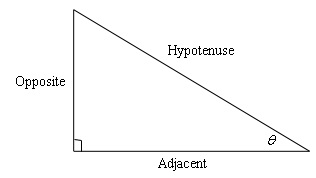
\includegraphics{RightTriangle.jpg}}

\centerline{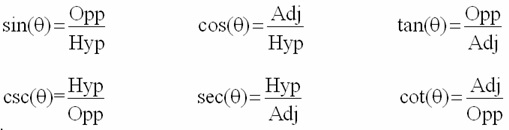
\includegraphics{TrigFunctionsTriangle.jpg}}

\centerline{\textbf{SOH-CAH-TOA}}
\vspace{2cm}
\textbf{Table of Common Values - Trig Functions:}

\centerline{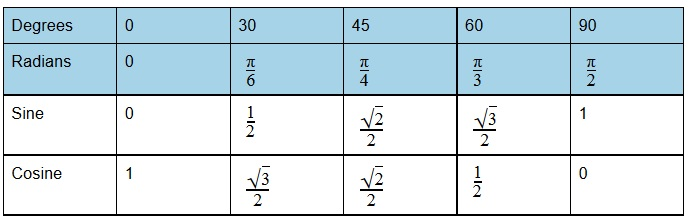
\includegraphics{TrigFunctionsCommonAngles.jpg}}

\newpage

\textbf{Unit Circle:}

\centerline{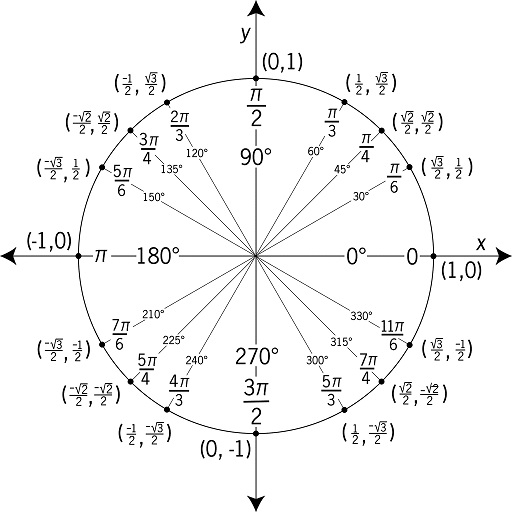
\includegraphics{UnitCircle.jpg}}

\newpage

\textbf{Signs of Trig Functions in Quadrants:}

\centerline{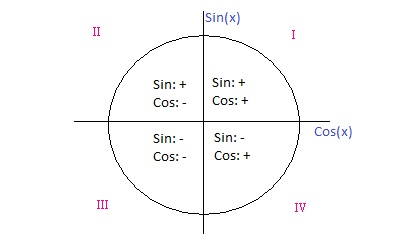
\includegraphics{QuadrantSignsTrigFunctions.jpg}}

\textbf{Even and Odd:}

\begin{enumerate}
\item \textbf{Cos(x)} is an \textbf{EVEN} function: $\cos(-x) = \cos(x)$ 

Graphically, $\cos(x)$ is symmetric about the y-axis
\item \textbf{Sin(x)} is an \textbf{ODD} function: $\sin(-x) = -\sin(x)$

Graphically, $\sin(x)$ is symmetric about the origin
\end{enumerate}

\newpage

\textbf{Reference Number} - for an real number $t$, the \textbf{reference number} $r$ associated with $t$ is the shortest distance along the unit circle from $t$ to the $x$-axis. For any $t$, the reference number $r$ is in $\Big[0, \dfrac{\pi}{2}\Big]$

\begin{myindentpar}{1cm}
\textbf{Example:} Determine the value of sin($t$) and cos($t$) for a) $t = \dfrac{29 \pi}{6}$ and b) $t = \dfrac{41 \pi}{4}$

\begin{myindentpar}{2cm}
\textbf{a)} First we find the reference number by finding the closest number to $29$ that evenly divides by $6$. We can use $30$. Then
\newline

\centerline{$\dfrac{29 \pi}{6} = \dfrac{30 \pi}{6} - \dfrac{\pi}{6}$}

So the reference number $r = \dfrac{\pi}{6}$. This helps us determine the value of sin(t) and cos(t). We know sin$\Big(\dfrac{\pi}{6}\Big)$ = $\dfrac{1}{2}$ and  cos$\Big(\dfrac{\pi}{6}\Big)$ = $\dfrac{\sqrt{3}}{2}$. We now just need to find what quadrant we are in to determine the correct sign.

So what quadrant are we in? $\dfrac{30 \pi}{6} = 5 \pi$ which places us at $(-1,0)$ on the unit circle. We then must move BACK (clockwise) $\dfrac{\pi}{6}$ radians which places us in the second quadrant where sin(t) is positive and cos(t) is negative.  

So sin$\Big(\dfrac{29 \pi}{6}\Big)$ = $\dfrac{1}{2}$ and  cos$\Big(\dfrac{29 \pi}{6}\Big)$ = $\dfrac{- \sqrt{3}}{2}$

\textbf{b)} First we find the reference number by finding the closest number to $41$ that evenly divides by $4$. We can use $40$. Then
\newline

\centerline{$\dfrac{41 \pi}{4} = \dfrac{40 \pi}{4} + \dfrac{\pi}{4}$}

So the reference number $r = \dfrac{\pi}{4}$. We know sin$\Big(\dfrac{\pi}{4}\Big)$ = $\dfrac{\sqrt{2}}{2}$ and  cos$\Big(\dfrac{\pi}{4}\Big)$ = $\dfrac{\sqrt{2}}{2}$

Now what quadrant are we in? $\dfrac{40 \pi}{4} = 10 \pi$ which places us at $(1,0)$ on the unit circle. We then must move FORWARD (counterclockwise) $\dfrac{\pi}{4}$ radians which places us in the first quadrant where sin(t) is positive and cos(t) is positive.

So sin$\Big(\dfrac{41 \pi}{4}\Big)$ = $\dfrac{\sqrt{2}}{2}$ and  cos$\Big(\dfrac{41 \pi}{4}\Big)$ = $\dfrac{\sqrt{2}}{2}$
\end{myindentpar}
\end{myindentpar}
\vspace{2cm}
\textbf{Graph of Sine:}

\centerline{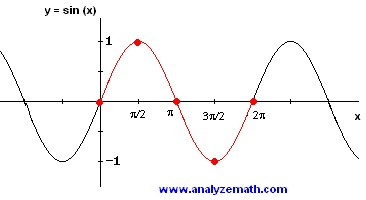
\includegraphics{SineGraph.jpg}}

\textbf{Graph of Cosine:}

\centerline{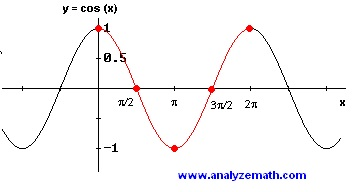
\includegraphics{CosineGraph.jpg}}

\newpage

\textbf{Graphs of $\mathbf{y = Asin(Bx + C) + D}$ and $\mathbf{y = Acos(Bx + C) + D}$}
\begin{itemize}
\item Amplitude: $|A|$
\item Period: $\dfrac{2 \pi}{B}$
\item Phase Shift: $\dfrac{|C|}{B}$

\begin{myindentpar}{2cm}
$\dfrac{C}{B} < 0 \implies$ shift right

$\dfrac{C}{B} > 0 \implies$ shift left
\end{myindentpar}

\item Interval: $\dfrac{2 \pi}{4B}$

\item Vertical Shift: $|D|$

\begin{myindentpar}{2cm}
$D < 0 \implies$ shift down

$D > 0 \implies$ shift up
\end{myindentpar}

\end{itemize}

\textbf{Note:} When graphing sine/cosine \textbf{phase shift} tells you how far left/right to move the first critical point. Then the \textbf{interval} tells you how far along the $x$-axis you go until the next critical point occurs. The \textbf{amplitude} tells you how far up/down you go for the maximum/minimum of the graphs. See notes on graphing sine and cosine uploaded onto Icon.


\textbf{The Other Trig Functions:}

\begin{enumerate}
\item tan($x$) = $\dfrac{\sin(x)}{\cos(x)}$
\item csc($x$) = $\dfrac{1}{\sin(x)}$
\item sec($x$) = $\dfrac{1}{\cos(x)}$
\item cot($x$) = $\dfrac{\cos(x)}{\sin(x)}$
\end{enumerate}

\newpage

\textbf{Graph of Tangent:}

\centerline{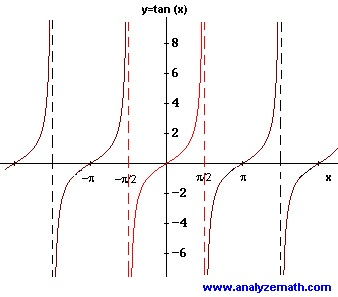
\includegraphics{TangentGraph.jpg}}

\textbf{Inverse Trig Functions:}

\begin{myindentpar}{1cm}
\begin{enumerate}

\item $\arcsin(x)$
\begin{myindentpar}{1cm}
\begin{enumerate}
\item $\sin\Big(\arcsin(x)\Big)$
\begin{myindentpar}{1cm}
\begin{enumerate}
\item $x$ in $[-1, 1]  \implies \sin\Big(\arcsin(x)\Big) = x$ 
\item  $x$  not in $[-1, 1] \implies$ \textbf{no solution}
\end{enumerate}
\end{myindentpar}
\item $\arcsin\Big(\sin(x)\Big)$
\begin{myindentpar}{1cm}
\begin{enumerate}
\item $x$ in $\Big[\dfrac{-\pi}{2}, \dfrac{\pi}{2}\Big] \implies \arcsin\Big(\sin(x)\Big) = x$ 
\item  $x$ not in $\Big[\dfrac{-\pi}{2}, \dfrac{\pi}{2}\Big] \implies$ find the corresponding radian measure that is inside $\Big[\dfrac{-\pi}{2}, \dfrac{\pi}{2}\Big]$
\end{enumerate}
\end{myindentpar}
\end{enumerate}
\end{myindentpar}

\item $\arccos(x)$
\begin{myindentpar}{1cm}
\begin{enumerate}
\item $\cos\Big(\arccos(x)\Big)$
\begin{myindentpar}{1cm}
\begin{enumerate}
\item $x$ in $[-1, 1] \implies \cos\Big(\arccos(x)\Big) = x$ 
\item  $x$ not in $[-1, 1] \implies $ \textbf{no solution}
\end{enumerate}
\end{myindentpar}
\item $\arccos\Big(\cos(x)\Big)$
\begin{myindentpar}{1cm}
\begin{enumerate}
\item $x$ in $[0, \pi] \implies \arccos\Big(\cos(x)\Big) = x$ 
\item  $x$ not in $[0, \pi] \implies $find the corresponding radian measure that is inside $[0, \pi]$
\end{enumerate}
\end{myindentpar}
\end{enumerate}
\end{myindentpar}

\item $\arctan(x)$
\begin{myindentpar}{1cm}
\begin{enumerate}
\item $\tan\Big(\arctan(x)\Big)$
\begin{myindentpar}{1cm}
\begin{enumerate}
\item $\tan\Big(\arctan(x)\Big) = x$ ALWAYS
\end{enumerate}
\end{myindentpar}
\item $\arctan\Big(\tan(x)\Big)$
\begin{myindentpar}{1cm}
\begin{enumerate}
\item $x$ in $\Big(\dfrac{-\pi}{2}, \dfrac{\pi}{2}\Big) \implies \arctan\Big(\tan(x)\Big) = x$ 
\item  $x$ not in $\Big(\dfrac{-\pi}{2}, \dfrac{\pi}{2}\Big) \implies$ find the corresponding radian measure that is inside $\Big(\dfrac{-\pi}{2}, \dfrac{\pi}{2}\Big)$
\end{enumerate}
\end{myindentpar}
\end{enumerate}
\end{myindentpar}

\end{enumerate}
\end{myindentpar}

\textbf{Law of Cosines:}

\centerline{$a^{2} = b^{2} + c^{2} - 2bc \cdot \cos(\alpha)$}

\textbf{Law of Sines:}

\centerline{$\dfrac{\sin(\alpha)}{a} = \dfrac{\sin(\beta)}{b} = \dfrac{\sin(\gamma)}{c}$}

\begin{myindentpar}{1cm}
\textbf{Note:} Remember when working with Law of Sines/Law of Cosines, the side opposite $\alpha$ is a, the side opposite $\beta$ is b and the side opposite $\gamma$ is c.

a $\rightarrow \alpha$

b $\rightarrow \beta$

c $\rightarrow \gamma$



\end{myindentpar}

\textbf{Heron's Formula:}

\centerline{$A = \sqrt{s(s-a)(s-b)(s-c)}$}

\vspace{1cm} 

\hspace{4cm} where $s = \dfrac{Perimeter}{2}$

\vspace{1cm}

\textbf{Exponential Function}
\newline

\centerline{$f(x) = a^x$ \hspace{2cm} $a\neq 1$} 

\vspace{.5cm}

\centerline{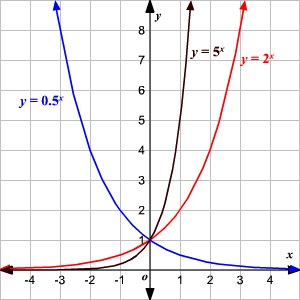
\includegraphics{ExponentialFunctionsAndGraphs.jpg}}

We say $a$ is the \textbf{base} of the exponential function.

There is a special kind of exponential function that we single out because of its significance and we call it the \textbf{Natural Exponential Function}. It is the function

\centerline{$f(x) = e^{x}$}

\newpage

\textbf{Logarithm Function}
\newline

\centerline{$f(x) = \log_{a}(x)$ \hspace{2cm} $a \neq 1$} 

\vspace{.5cm}

\centerline{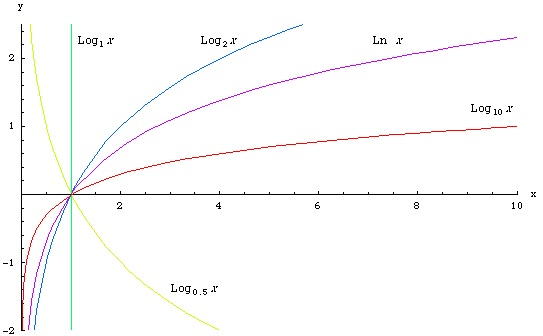
\includegraphics{LogGraph.jpg}}

Again, we call $a$ the \textbf{base} of the logarithm function. 

There is a special kind of logarithm function that we single out becaue of its significance. It is the \textbf{Natural Log Function}. It is the function
\newline

\centerline{$f(x) = \ln(x)$}

The Natural Log Function is the logarithm function with \textbf{base e} ($f(x) = \log_{e}(x)$) and it is the \textbf{inverse} of the natural exponential function $f(x) = e^{x}$

\textbf{Note:} If you see something like $f(x) = \log(x)$ with no base, then we assume it is \textbf{log base 10}, or written out, we assume $f(x) = \log_{10}(x)$

\textbf{Evaluating Logarithms:}

\begin{myindentpar}{1cm}

\textbf{Evaluate the following expressions:}

\begin{enumerate}
\item $\log_{2}(8)$ 
\item $\log_{32}(2)$
\item $\log_{7}(-3)$
\item $6^{\log_{6}(8)}$

\end{enumerate}

\textbf{(1)} We ask ourselves the following question: When does $2^{y} = 8$? Well we know $2^{3} = 8$ so our answer is $\log_{2}(8) = 3$ 

\textbf{(2)} We ask ourselves the following question: When does $32^{y} = 2$? Well we know $32^{\dfrac{1}{5}} = 2$ so our answer is $\log_{32}(2) = \dfrac{1}{5}$ 

\textbf{(3)} We ask ourselves the following question: When does $7^{y} = -3$? If we think about it we should realize this can never happen so there is no solution

\textbf{(4)} There is a property in the book that says that $a^{\log_{a}(x)} = x$ so our answer is $6^{\log_{6}(8)} = 8$
\end{myindentpar}

\vspace{1cm}

\textbf{Important Properties of Logs:}
\begin{myindentpar}{2cm}
\begin{enumerate}
\item $\log(x \cdot y) = \log(x) + \log(y)$ 
\item $\log\Big(\dfrac{x}{y}\Big) = \log(x) - \log(y)$
\item $\log(x^{p}) = p \cdot \log(x)$
\end{enumerate}
\end{myindentpar}

\vspace{1cm}

\textbf{Graph Translations:}

\begin{myindentpar}{2cm}

\textbf{Vertical Shifts:} Let $c>0$

\begin{enumerate}
\item $y=f(x) + c$ shifts $f(x)$ c units up
\item $y=f(x) - c$ shifts $f(x)$ c units down
\end{enumerate}

\textbf{Horizontal Shifts:} Let $c>0$

\begin{enumerate}
\item $y=f(x+c)$ shifts $f(x)$ c units left
\item $y=f(x-c)$ shifts $f(x)$ c units right
\end{enumerate}

\textbf{Reflections:} 

\begin{enumerate}
\item $y=-f(x)$ reflects $f(x)$ about the x-axis
\item $y=f(-x)$ reflects $f(x)$ about the y-axis
\end{enumerate}

\textbf{Vertical Stretch \& Shrink:} 
\newline

\centerline{Let $c>0$. We consider $y=cf(x)$}

\begin{enumerate}
\item $c>1 \hspace{.75cm} \to$ stretch $f(x)$ vertically by a factor of c
\item $0<c<1 \to$ shrink $f(x)$ vertically by a factor of c
\end{enumerate}
\vspace{.5cm}
\textbf{Horizontal Stretch \& Shrink:} 
\newline

\centerline{Let $c>0$. We consider $y=f(cx)$}

\begin{enumerate}
\item $c>1 \hspace{.75cm} \to$ shrink $f(x)$ horizontally by a factor of c
\item $0<c<1 \to$ stretch $f(x)$ horizontally by a factor of c
\end{enumerate}
\end{myindentpar}

\textbf{Compount Interest Formulas:}

\begin{myindentpar}{2cm}

\begin{itemize}
\item \textbf{Non-Continuous Compounding}
\newline

\centerline{$A = A_{0}\Big(1+ \dfrac{r}{n}\Big)^{nt}$}


\item \textbf{Continuous Compounding}
\newline

\centerline{$A = A_{0}e^{rt}$}

\end{itemize}

$A$ = Amount

$A_{0}$ = Principal

$r$ = Interest rate

$n$ = Number of times compounded per year

$t$ = Time
\end{myindentpar}


























\end{document}